\documentclass{beamer}

\usetheme{Warsaw}

\usepackage[utf8]{inputenc}
\usepackage[frenchb]{babel}
\usepackage[T1]{fontenc}
\usepackage{amsmath}
\usepackage{hyperref}

\usepackage{graphicx}

\usepackage{tikz}
\usetikzlibrary{arrows}

\pdfcompresslevel0

\usepackage{color}

\addtobeamertemplate{footline}{\hfill\insertframenumber/\inserttotalframenumber

\hspace{10em}\\}

\usepackage{listings}

\title{Interopérabilité entre OCaml et Java }
\author{Béatrice Carré}
\date{\today}

% slides number
\defbeamertemplate*{footline}{shadow theme}
{%
  \leavevmode%
  \hbox{
    \begin{beamercolorbox}[wd=.5\paperwidth,ht=2.5ex,dp=1.125ex,leftskip=.3cm plus1fil,rightskip=.3cm]{author in head/foot}%
    \usebeamerfont{author in head/foot}\insertframenumber\,/\,\inserttotalframenumber\hfill\insertshortauthor
  \end{beamercolorbox}%
  \begin{beamercolorbox}[wd=.5\paperwidth,ht=2.5ex,dp=1.125ex,leftskip=.3cm,rightskip=.3cm plus1fil]{}%
    \usebeamerfont{title in head/foot}\insertshorttitle%
  \end{beamercolorbox}}%
  \vskip0pt%
}

\beamertemplatenavigationsymbolsempty


\begin{document}

\maketitle





\begin{frame}{Objectif}

Caractéristiques d'une interopérabilité efficace :
\begin{itemize}
\item accès à l'autre monde simple ou implicite
\item bonne gestion mémoire et des exceptions
\item gestion des caractéristiques de chaque monde
\end{itemize}

\end{frame}



\begin{frame}{Comparaison des deux mondes}
  
L'interopérabilité se fait sur le modèle objet de chacun

\bigskip
\begin{tabular}{|l|c|c|c|c|}
  \hline
  \emph{caractéristiques} & \emph{Java} & \emph{OCaml} \\
  \hline
  accès champs & selon la visibilité & via appels de méthode\\\hline
  var./méth. statiques & \checkmark & fonct./décl. globales\\\hline
  typage dynamique & \checkmark & pas de downcast \\\hline
  héritage$\equiv$sous-typage? &\checkmark  & $\times$ \\\hline
  surcharge & \checkmark & $\times$ \\\hline
  héritage multiple & pour les interfaces & \checkmark\\
  \hline
  modules paramétrés & $\times$ & \checkmark\\\hline
\end{tabular}

\bigskip

$\Rightarrow$ Il faut réduire les possibilités d'un outil à l'intersection des deux mondes
 
\end{frame}




\begin{frame}{O'Jacaré : schéma global }

Pour un accès à des classes Java :

O'Jacaré génère leurs classes encapsulantes à partir d'un fichier dans lequel sont décrites les classes qu'on veut manipuler.
\medskip
\begin{figure}[h]
  \centering
  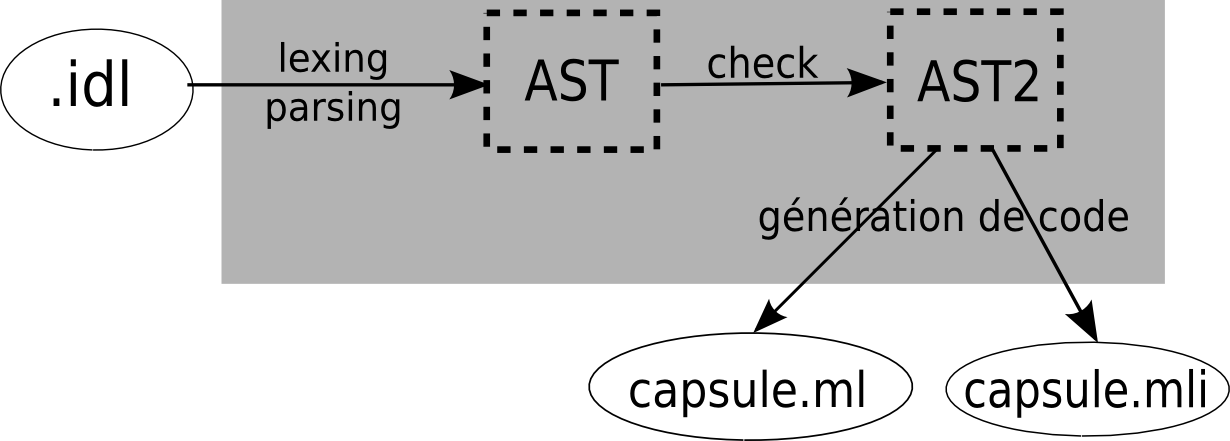
\includegraphics[scale=0.6]{schemaOjacare.png}
  \caption{La génération de code d'O'Jacaré}
\end{figure}

\end{frame}





\begin{frame}{O'Jacaré : schéma global }
\begin{itemize}
\item La capsule générée permet à l'utilisateur de faire des appels transparents à des méthodes Java.
\item Camljava gère la communication entre les deux mondes :
\begin{itemize}
\item Recherche des classes par nom et des méthodes par signature
\item Conversion des types de base est assurée
\end{itemize}
\end{itemize}
\begin{figure}[h]
  \centering
  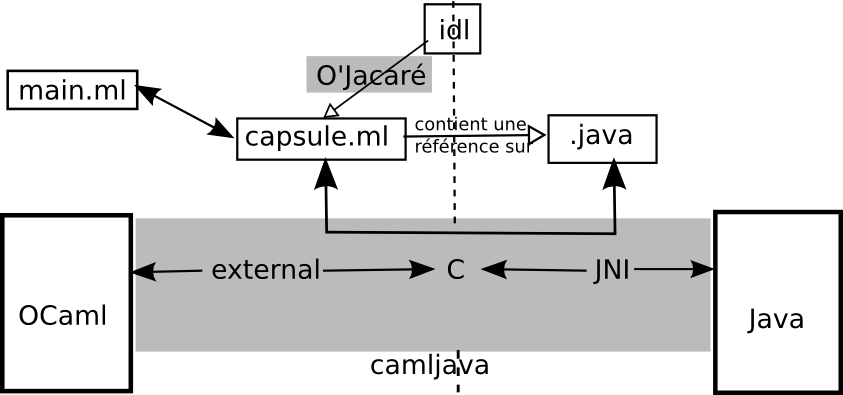
\includegraphics[scale=0.6]{schemaCamljava2.png}
\end{figure}

\end{frame}







\begin{frame}{O'Jacaré : exemple d'idl}
  
\begin{figure}[h]
  \centering
  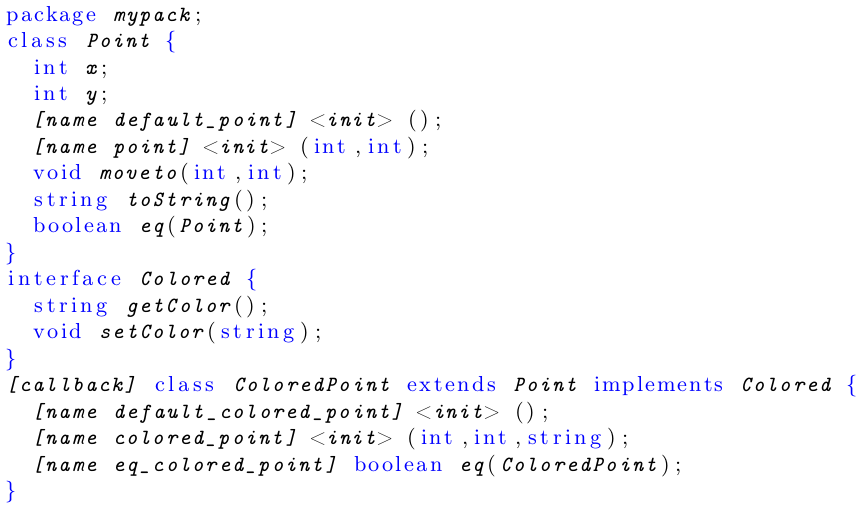
\includegraphics[scale=0.35]{pointIdlEx.png}
\end{figure}
\end{frame}




\begin{frame}{OCaml-Java : schéma global}
\begin{figure}
  \centering
  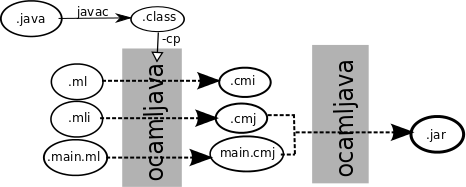
\includegraphics[scale=0.5]{schemaOCamlJava.png}
\end{figure}
Compilation vers du bytecode Java

$\Rightarrow$ un seul runtime
Pas de problème de gestion mémoire, de communications .
\end{frame}





\begin{frame}{OCaml-Java : l'accès au monde Java}
\begin{figure}[h]
  \centering
  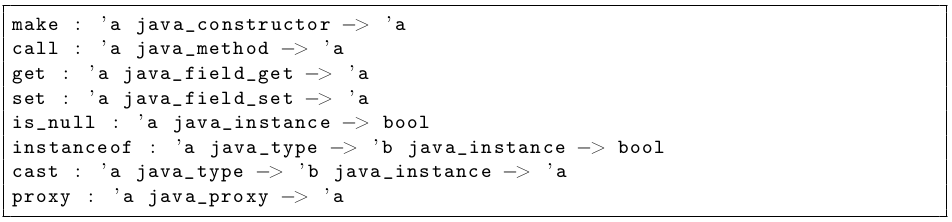
\includegraphics[scale=0.33]{methModuleJava.png}
\end{figure}

Accès à l'API Java et à du code utilisateur grâce à ce module.
\begin{figure}[h]
  \centering
  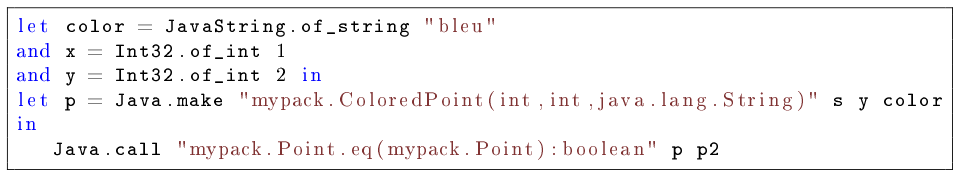
\includegraphics[scale=0.30]{exempleOCaml-Java.png}
\end{figure}

\end{frame}


\begin{frame}{Fusion des deux approches}

\begin{tabular}{|c|c|c|}
  \hline
   \emph{O'Jacaré+CamlJava} & \emph{OCaml-Java} & \emph{O'Jacaré+OCaml-Java}\\
  \hline
  appels transparents & via module Java & appels transparents\\\hline
  2 runtime & 1 runtime & 1 runtime \\\hline
  Pas d'allocation & & \\\hline
  vérifications accès & vérifications accès & vérifications accès \\
  dans la capsule & par le compilateur & par le compilateur\\
  (avant accès Java) & (côté Java) & (côté Java) \\ \hline
\end{tabular}

\end{frame}


\begin{frame}{Adaptation d'Ojacaré}

\begin{figure}[h]
  \centering
  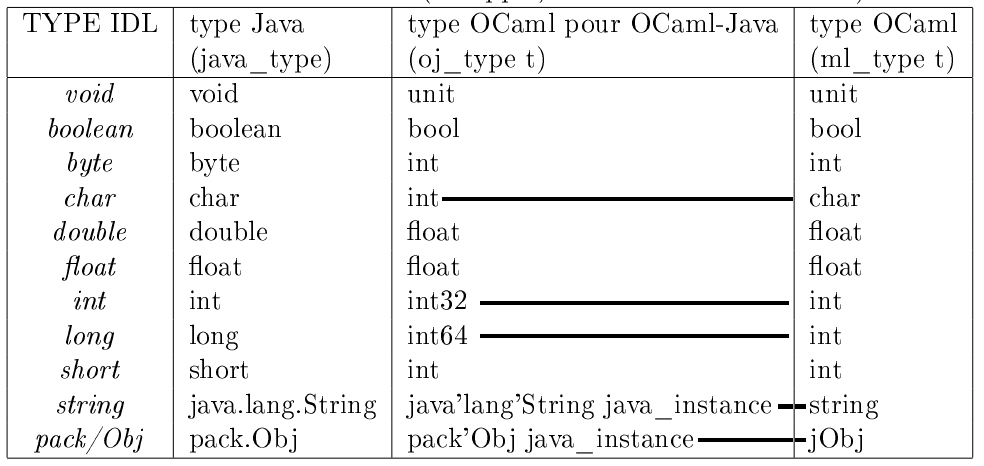
\includegraphics[scale=0.30]{typesOCamlJava.png}
  \caption{Les types dans OCamlJava}
\end{figure}

\end{frame}

\begin{frame}{Comparaison de génération}
\begin{figure}[h]
  \centering
  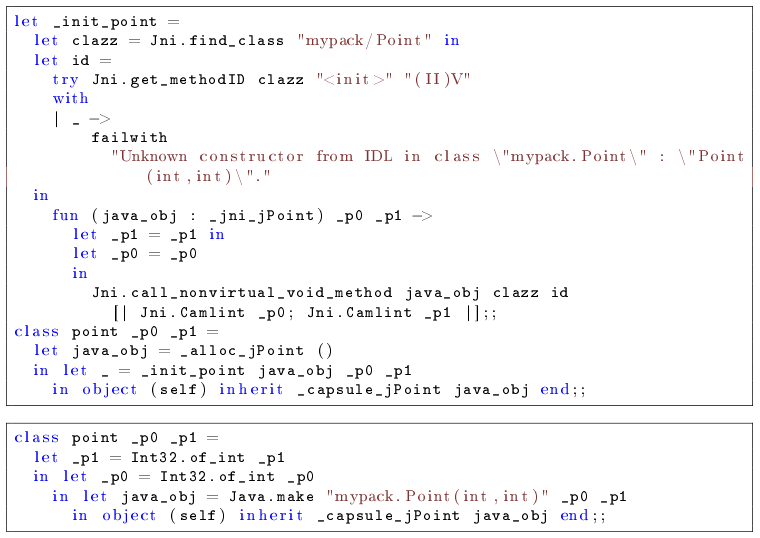
\includegraphics[scale=0.35]{exemple.png}
  \caption{La génération du constructeur de Point}
\end{figure}
\end{frame}


\begin{frame}{Conclusion}

Ce nouvel outil a apporté des nouvelles possibilités d'un côté,
avec une simplicité d'utilisation :
\begin{itemize}
\item Accès simple à l'API Java
\item Accès utilisateur transparent grâce aux classes encapsulantes
\item 1 seul runtime -> Gestion mémoire simplifiée et sûre
\item Code généré simplifié ($\sim$ 5 fois moins)
\item 
\end{itemize}

\begin{tabular}{|l|c|}
  \hline
  \emph{caractéristiques} & \emph{O'Jacaré + OCaml-Java} \\
  \hline
  accès champs & selon la visibilité + via appels de méthode\\\hline
  var./méth. statiques &  fonctions/décl. globales\\\hline
  héritage$\equiv$sous-typage? & $\times$ \\\hline
  surcharge & $\times$ \\\hline
  héritage multiple & \checkmark\\
  \hline
\end{tabular}


\end{frame}

%% \begin{frame}{Bibliographie}
  
%%   \begin{thebibliography}{9}
%%   \bibitem{amato2013localizing}
%%     Amato, Gianluca and Scozzari, Francesca,
%%     \emph{Localizing widening and narrowing}.
%%     Static Analysis, Springer.
%%     pages 25--42,
%%     2013.

%%   \bibitem{halbwachs2012decreasing}
%%     Halbwachs, Nicolas and Henry, Julien,
%%     \emph{When the decreasing sequence fails}.
%%     Static Analysis, Springer.
%%     pages 198--213,
%%     2012.
%%   \end{thebibliography}

%% \end{frame}

\end{document}

